\newpage
\section{Introduction}
\label{sec:introduction}
% state the learning objective 

The objective of this laboratory assignment is to choose the best architecture of the Gain and Output amplifier
stages in order to build an audio amplifier. This assignment allowed us to deal with important concepts such as BJTs Transistors and its diverse utility in circuits. We did this while paying attention to the merit of the project designed.\\
This merit is calculated exactly as the next equation:

\begin{equation} 
M = \frac{voltageGain*bandwidth}{cost*lowerCutoffFreq}
\label{eq1}
\end{equation}

Being the cost the following:
\begin{itemize}
	\item cost = cost of resistors  + cost of capacitors + cost of transistors
	\item cost of resistors = 1 monetary unit (MU) per kOhm
	\item cost of capacitors = 1 MU/$\mu$F
	\item cost of diodes = 0.1 MU per transistor
	
\end{itemize}

\begin{figure}[H] 
\centering
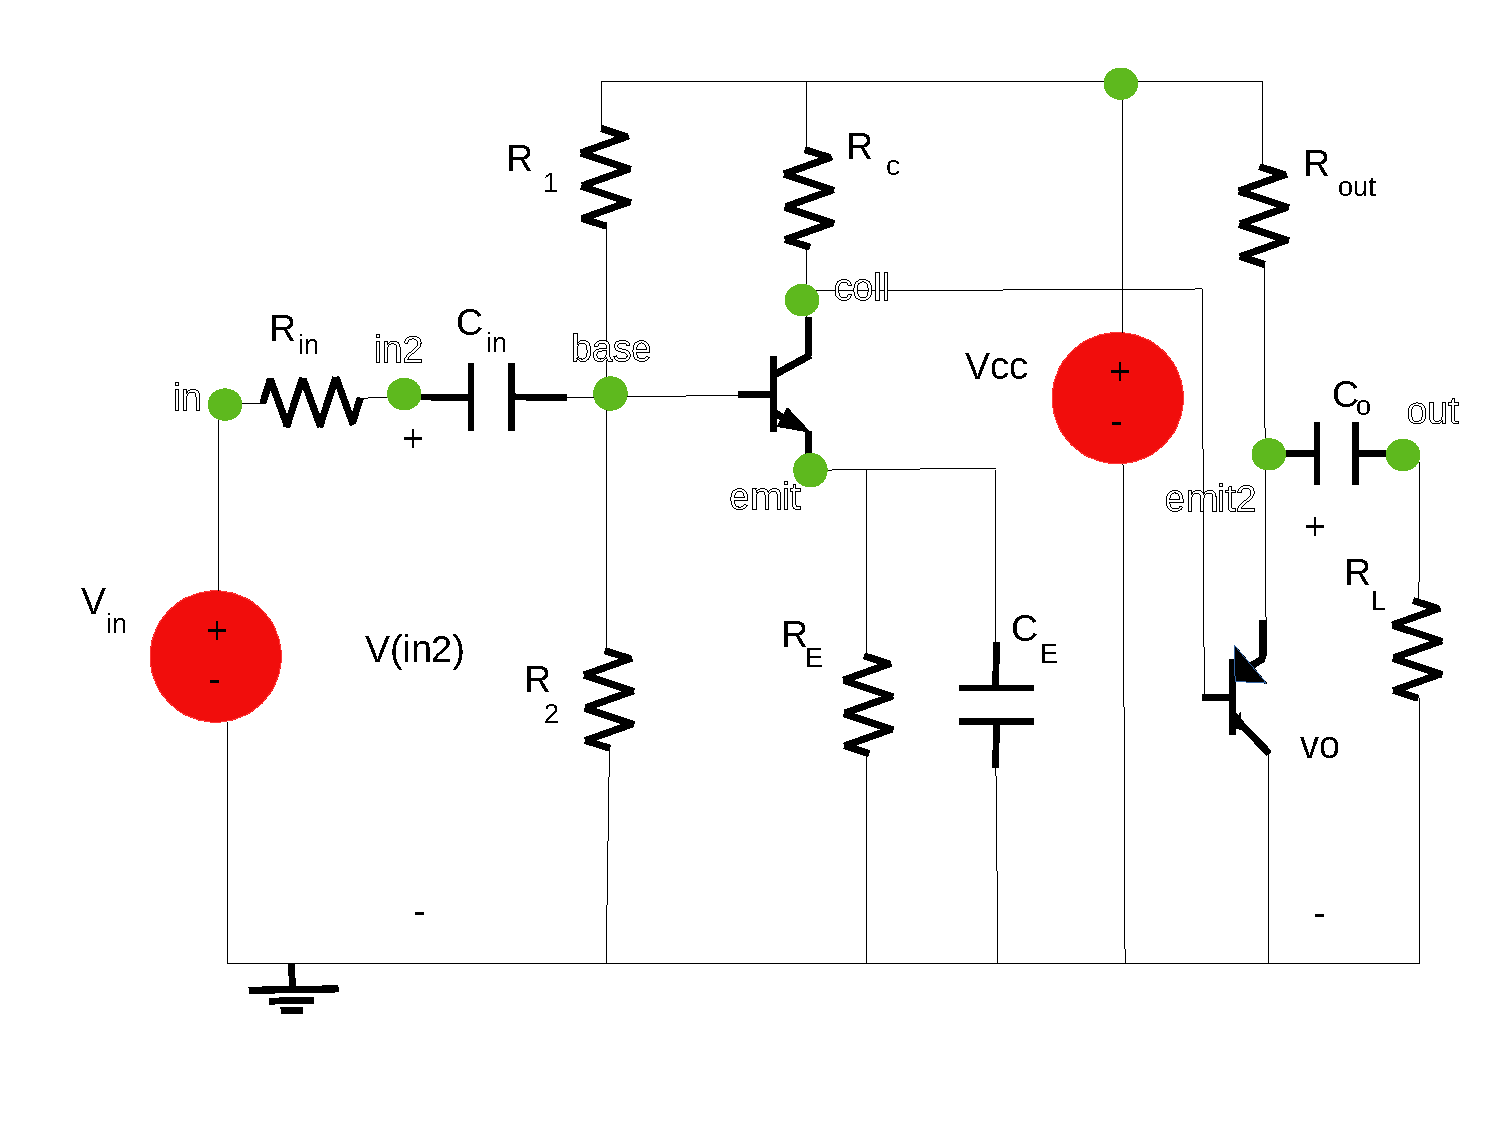
\includegraphics[width=\textwidth]{lab4.pdf} 
\caption{Audio Amplifier}
\label{first}
\end{figure}

To obtain the best values for the circuit, we've used the matlab simulink to optimize them for the best merit.

In Section~\ref{sec:analysis}, a theoretical analysis of the circuit is
presented. In Section~\ref{sec:simulation}, the circuit is analysed by
simulation, and the results are compared to the theoretical results obtained in
Section~\ref{sec:analysis}. The conclusions of this study are outlined in
Section~\ref{sec:conclusion}. \\


